\section{Bab 1 Pendahuluan}
\subsection{Latar Belakang}
\begin{frame}
\frametitle{BAB 1 Pendahuluan}
\begin{block}<1->{Latar Belakang}
\begin{figure}[H]
\centering
%Definisi
\tikzstyle{kotak} = [rectangle, minimum height=2cm, text width=3cm, text centered, draw=black, fill=blue!30]
\tikzstyle{garis} = [thick,->,>=stealth]
%Gambar
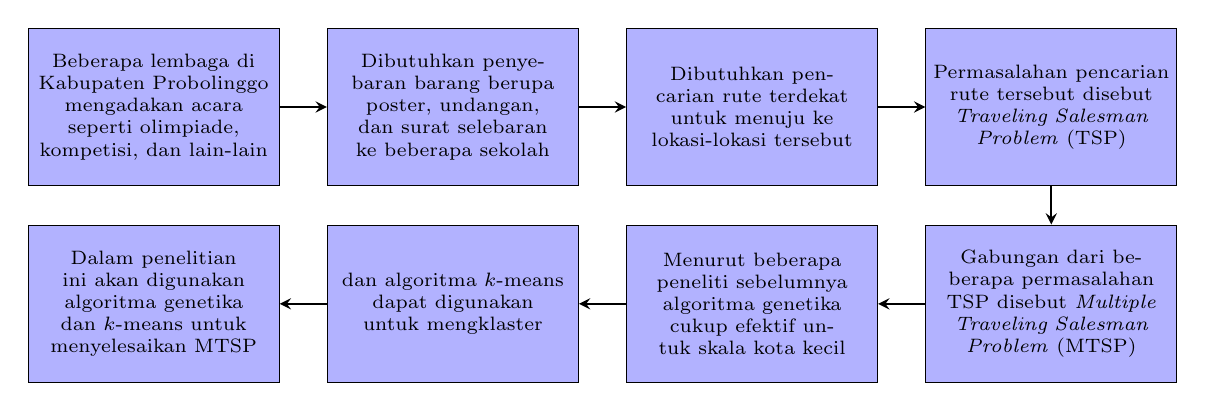
\begin{tikzpicture}
\scriptsize
\onslide<2-> \node (1) [kotak] {Beberapa lembaga di Kabupaten Probolinggo mengadakan acara seperti olimpiade, kompetisi, dan lain-lain};
\onslide<3-> \node (2) [kotak, right of=1, xshift=+2.8cm]{Dibutuhkan penyebaran barang berupa poster, undangan, dan surat selebaran ke beberapa sekolah};
\onslide<4->  \node (3) [kotak, right of=2, xshift=+2.8cm]{Dibutuhkan pencarian rute terdekat untuk menuju ke lokasi-lokasi tersebut};
\onslide<5->  \node (4) [kotak, right of=3, xshift=+2.8cm]{Permasalahan pencarian rute tersebut disebut \textit{Traveling Salesman Problem} (TSP)};
\onslide<6-> \node (5) [kotak, below of=4, yshift=-1.5cm]{Gabungan dari beberapa permasalahan TSP disebut \textit{Multiple Traveling Salesman Problem} (MTSP)};
\onslide<7-> \node (6) [kotak, left of=5, xshift=-2.8cm]{Menurut beberapa peneliti sebelumnya algoritma genetika cukup efektif untuk skala kota kecil};
\onslide<8-> \node (7) [kotak, left of=6, xshift=-2.8cm]{dan algoritma $k$-means dapat digunakan untuk mengklaster};
\onslide<9-> \node (8) [kotak, left of=7, xshift=-2.8cm]{Dalam penelitian ini akan digunakan algoritma genetika dan $k$-means untuk menyelesaikan MTSP};

\onslide<2-> \draw [garis] (1) -- (2);
\onslide<3-> \draw [garis] (2) -- (3);
\onslide<4-> \draw [garis] (3) -- (4);
\onslide<5-> \draw [garis] (4) -- (5);
\onslide<6-> \draw [garis] (5) -- (6);
\onslide<7-> \draw [garis] (6) -- (7);
\onslide<8-> \draw [garis] (7) -- (8);
\end{tikzpicture}
\end{figure}
\end{block}
\end{frame}

\subsection{Tujuan Penelitian}
\subsection{Manfaat Penelitian}

\begin{frame}
\frametitle{BAB 1 Pendahuluan}
\begin{block}<1->{Tujuan Penelitian}
\begin{enumerate}
\item<2-> Mengetahui cara menemukan solusi \textit{Multiple Travelling Salesman Problem} menggunakan algoritma genetika dan $k$-means.
\item<3-> Menemukan solusi pembagian klaster dan urutan jalur terdekat menuju seluruh SMA di Kabupaten Probolinggo.
\end{enumerate}
\end{block}

\begin{block}<4->{Manfaat Penelitian}
\begin{enumerate}
\item<5-> satu
\item<6-> dua
\end{enumerate}
\end{block}
\end{frame}